%!TEX encoding=UTF-8 Unicode
% Palette Dark2 3 colors
\definecolor{ColF}{HTML}{1B9E77}
\definecolor{ColV}{HTML}{D95F02}
\definecolor{ColM}{HTML}{7570B3}



\tikzset{
    % Args: BeginVal, EndVal, Size, label, Color
    pics/access/.style args={#1#2#3#4#5}{
        code={
            \draw[|-|,thick,#5] (0,0) node[pos=0,below=2pt,#5]{#1} -- (#3,0)
            node[pos=1,below=2pt,#5]{#2};
            \node[ColV][anchor=south] at (#3/2,0) {#4};
        }
    },
}
\tikzstyle{mybrace} = [decorate,decoration={brace, mirror,amplitude=1em},thick]

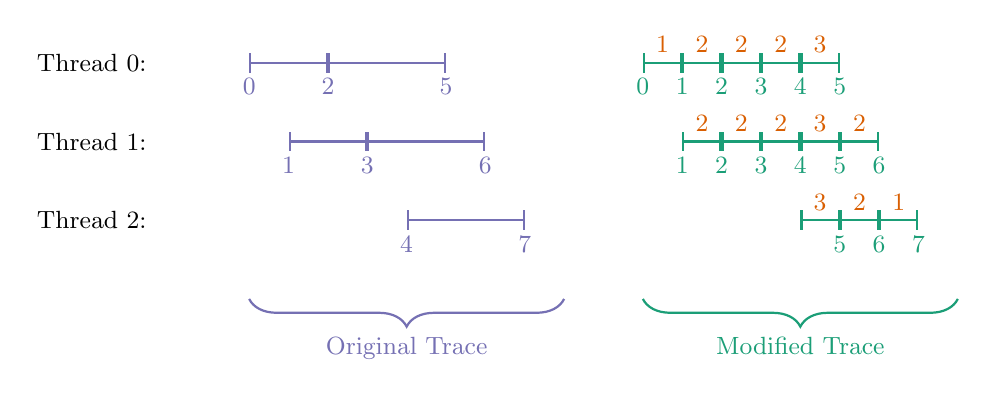
\begin{tikzpicture}[font=\small]
    \node at (-2,0) {Thread 0:};
    \node at (-2,-1) {Thread 1:};
    \node at (-2,-2) {Thread 2:};

    \draw[mybrace,ColM] (0,-3) -- (4,-3) node[pos=.5,below=1em] {Original Trace};
    \draw[mybrace,ColF] (5,-3) -- (9,-3) node[pos=.5,below=1em] {Modified Trace};

    % Moca trace
    \pic at (0,0)       {access={0}{2}{1}{}{ColM}};
    \pic at (1,0)       {access={ }{5}{1.5}{}{ColM}};

    \pic at (0.5,-1)    {access={1}{3}{1}{}{ColM}};
    \pic at (1.5,-1)    {access={ }{6}{1.5}{}{ColM}};

    \pic at (2,-2)      {access={4}{7}{1.5}{}{ColM}};

    % After parsing
    \pic at (5,0)       {access={0}{1}{.5}{1}{ColF}};
    \pic at (5.5,0)     {access={ }{2}{.5}{2}{ColF}};
    \pic at (6,0)       {access={ }{3}{.5}{2}{ColF}};
    \pic at (6.5,0)     {access={ }{4}{.5}{2}{ColF}};
    \pic at (7,0)       {access={ }{5}{.5}{3}{ColF}};

    \pic at (5.5,-1)    {access={1}{2}{.5}{2}{ColF}};
    \pic at (6,-1)      {access={ }{3}{.5}{2}{ColF}};
    \pic at (6.5,-1)    {access={ }{4}{.5}{2}{ColF}};
    \pic at (7,-1)      {access={ }{5}{.5}{3}{ColF}};
    \pic at (7.5,-1)    {access={ }{6}{.5}{2}{ColF}};

    \pic at (7,-2)      {access={ }{5}{.5}{3}{ColF}};
    \pic at (7.5,-2)    {access={ }{6}{.5}{2}{ColF}};
    \pic at (8,-2)      {access={ }{7}{.5}{1}{ColF}};
\end{tikzpicture}
% vim: et si sta lbr  sw=4 ts=4 spelllang=en_us
